\typeout{Reducing Disclosed Dependencies in Privacy Preserving Planning}

% These are the instructions for authors for IJCAI-21.

\documentclass{article}
\pdfpagewidth=8.5in
\pdfpageheight=11in
% The file ijcai21.sty is NOT the same than previous years'
\usepackage{ijcai21}

% Use the postscript times font!
\usepackage{times}
\usepackage{soul}
\usepackage{url}
\usepackage[hidelinks]{hyperref}
\usepackage[utf8]{inputenc}
\usepackage[small]{caption}
\usepackage{graphicx}
\usepackage{amsmath}
\usepackage{amsthm}
\usepackage{booktabs}
%\usepackage{algorithm}
\usepackage{algorithmic}
\usepackage[ruled,linesnumbered,noend]{algorithm2e}
\urlstyle{same}

% the following package is optional:
%\usepackage{latexsym}

% See https://www.overleaf.com/learn/latex/theorems_and_proofs
% for a nice explanation of how to define new theorems, but keep
% in mind that the amsthm package is already included in this
% template and that you must *not* alter the styling.
\newtheorem{example}{Example}
\newtheorem{theorem}{Theorem}
\newtheorem{observation}{Observation}
\newtheorem{corollary}{Corollary}


% Following comment is from ijcai97-submit.tex:
% The preparation of these files was supported by Schlumberger Palo Alto
% Research, AT\&T Bell Laboratories, and Morgan Kaufmann Publishers.
% Shirley Jowell, of Morgan Kaufmann Publishers, and Peter F.
% Patel-Schneider, of AT\&T Bell Laboratories collaborated on their
% preparation.

% These instructions can be modified and used in other conferences as long
% as credit to the authors and supporting agencies is retained, this notice
% is not changed, and further modification or reuse is not restricted.
% Neither Shirley Jowell nor Peter F. Patel-Schneider can be listed as
% contacts for providing assistance without their prior permission.

% To use for other conferences, change references to files and the
% conference appropriate and use other authors, contacts, publishers, and
% organizations.
% Also change the deadline and address for returning papers and the length and
% page charge instructions.
% Put where the files are available in the appropriate places.

%File: formatting-instruction.tex
%\documentclass[sigconf]{aamas} 
%\documentclass[sigconf,anonymous]{aamas}

%\usepackage{balance}
% Below is not from AAMAS:
%\usepackage{times}  %Required
\usepackage{helvet}  %Required
\usepackage{courier}  %Required
%\usepackage{url}  %Required
%\usepackage{graphicx}  %Required

\usepackage{multirow}
%\usepackage[table,xcdraw]{xcolor}
%\usepackage{booktabs}
%\usepackage{amsmath,amssymb}
%\usepackage{eurosym}
% Use the postscript times font!
%\usepackage{times}
%\usepackage{mathtools}
%\usepackage{soul}
%\usepackage{url}
%\usepackage[hidelinks]{hyperref}
%\usepackage[utf8]{inputenc}
%\usepackage[small]{caption}
%\usepackage{graphicx}
%\usepackage{amsmath}
%\usepackage{amsfonts}
%\usepackage{amssymb}
%\usepackage{amsthm}
%\usepackage{booktabs}
%\usepackage[ruled,linesnumbered,noend]{algorithm2e}
%\usepackage{amsthm}   
%\usepackage{pgfplots,graphicx}
\usepackage{subcaption}
% Use the postscript times font!
%%\usepackage{times}
%\usepackage{soul}
%\usepackage{url}
%\usepackage[hidelinks]{hyperref}
%\usepackage[utf8]{inputenc}
%\usepackage{graphicx}
%\usepackage{amsmath}
%\usepackage{booktabs}
%\usepackage{algorithmic}
%\usepackage{thmtools}
\usepackage{xcolor}

\newtheorem{definition}{Definition}



\setlength{\intextsep}{5pt} % Vertical space above & below [h] floats
\setlength{\textfloatsep}{5pt} % h space below (above) [t] ([b]) floats
\setlength{\abovecaptionskip}{10pt}
\setlength{\belowcaptionskip}{0pt}

\usepackage{xspace}
\newcommand{\cppp}{\textsc {cppp}\xspace}
\newcommand{\mafs}{\textsc {mafs}\xspace}
\newcommand{\smafs}{\textsc {smafs}\xspace}
\newcommand{\fmafs}{\textsc {mafbs}\xspace}
\newcommand{\mafbs}{\textsc {mafbs}\xspace}
\newcommand{\smafbs}{\textsc {smafbs}\xspace}
\newcommand{\mastrips}{\textsc {ma-strips}\xspace}
\newcommand{\dpp}{\textsc {DPP}\xspace}

\newcommand{\psolve}{\ensuremath{P_{solve}}\xspace}
\newcommand{\commentout}[1]{}


\urlstyle{same}
\usepackage{array}
\newcolumntype{L}{>{\centering\arraybackslash}m{3cm}}
\newcommand{\rotem}[1]{\textbf{\color{red}[ROTEM:#1]}}
\newcommand{\rotemNew}[1]{\textbf{\color{purple}[ROTEM New:#1]}}
\newcommand{\roni}[1]{\textbf{\color{blue}[RONI:#1]}}
\newcommand{\guy}[1]{\textbf{\color{orange}[GUY:#1]}}

% \newcommand{\rotem}[1]{ }
% \newcommand{\rotemNew}[1]{ }
% \newcommand{\roni}[1]{}
% \newcommand{\guy}[1]{}

\commentout{
\declaretheorem{theorem} 
\declaretheoremstyle[%
  spaceabove=0pt,%
  spacebelow=0pt,%
  headfont=\normalfont\itshape,%
  postheadspace=1em,%
  qed=\qedsymbol%
]{mystyle} 
\declaretheorem[name={Proof},style=mystyle,unnumbered,
]{prf}
}
\usepackage{adjustbox}

\theoremstyle{remark}
\newtheorem{definition1}{Definition}
%\newtheorem{example}{Example}
\newtheorem{lemma}{Lemma}
\newtheorem{proposition}{Proposition}
\newcolumntype{R}[2]{%
    >{\adjustbox{angle=#1,lap=\width-(#2)}\bgroup}%
    l%
    <{\egroup}%
}

\newcommand*\rot{\multicolumn{1}{R{45}{1em}}}
\newcommand{\citet}[1]{\citeauthor{#1}~\shortcite{#1}}
\newcommand{\citep}[1]{\cite{#1}}


\newcommand{\move}[0]{\mbox{{\em move}}}
% the following package is optional:
%\usepackage{latexsym} 


%\setcounter{secnumdepth}{2}


%%% AAMAS-2021 copyright block (do not change!)

%\setcopyright{ifaamas}
%\acmConference[AAMAS '21]{Proc.\@ of the 20th International Conference on Autonomous Agents and Multiagent Systems (AAMAS 2021)}{May 3--7, 2021}{London, UK}{U.~Endriss, A.~Now\'{e}, F.~Dignum, A.~Lomuscio (eds.)}
%\copyrightyear{2021}
%\acmYear{2021}
%\acmDOI{}
%\acmPrice{}
%\acmISBN{}

%%%%%%%%%%%%%%%%%%%%%%%%%%%%%%%%%%%%%%%%%%%%%%%%%%%%%%%%%%%%%%%%%%%%%%%%

%%% Use this command to specify your EasyChair submission number.
%%% In anonymous mode, it will be printed on the first page.

%\acmSubmissionID{588}

%%% Use this environment to specify a short abstract for your paper.
%\author{Rotem Lev Lehman, Guy Shani, Roni Stern}

% \author{Rotem Lev Lehman \and Guy Shani \and Roni Stern\\ % All authors must be in the same font size and format. Use \Large and \textbf to achieve this result when breaking a line
% Software and Information Systems Engineering\\ %If you have multiple authors and multiple affiliations
% % use superscripts in text and roman font to identify them. For example, Sunil Issar,\textsuperscript{\rm 2} J. Scott Penberthy\textsuperscript{\rm 3} George Ferguson,\textsuperscript{\rm 4} Hans Guesgen\textsuperscript{\rm 5}. Note that the comma should be placed BEFORE the superscript for optimum readability
% Ben Gurion University, Israel \\
% \texttt{levlerot@post.bgu.ac.il}, \texttt{shanigu@bgu.ac.il}, \texttt{sternron@post.bgu.ac.il}
% % email address must be in roman text type, not monospace or sans serif
% }
\commentout{
\author{Rotem Lev Lehman\textsuperscript{\rm 1} \and Guy Shani\textsuperscript{\rm 1} \and Roni Stern\textsuperscript{\rm 1,2} \\ % All authors must be in the same font size and format. Use \Large and \textbf to achieve this result when breaking a line
% Software and Information Systems Engineering\\ %If you have multiple authors and multiple affiliations
% % use superscripts in text and roman font to identify them. For example, Sunil Issar,\textsuperscript{\rm 2} J. Scott Penberthy\textsuperscript{\rm 3} George Ferguson,\textsuperscript{\rm 4} Hans Guesgen\textsuperscript{\rm 5}. Note that the comma should be placed BEFORE the superscript for optimum readability
% Ben Gurion University, Israel \\
% email address must be in roman text type, not monospace or sans serif
\textsuperscript{\rm 1}Software and Information Systems Engineering, Ben Gurion University of the Negev, Be'er Sheva, Israel\\
\textsuperscript{\rm 2}Palo Alto Research Center, Palo Alto, CA, USA\\
levlerot@post.bgu.ac.il, shanigu@bgu.ac.il, sternron@post.bgu.ac.il \\
}
}


%PDF Info Is REQUIRED.
\pdfinfo{
/TemplateVersion (IJCAI.2021.0)
}

\title{Reducing Disclosed Dependencies in Privacy Preserving Planning}


% Multiple author syntax (remove the single-author syntax above and the \iffalse ... \fi here)
% Check the ijcai21-multiauthor.tex file for detailed instructions

\commentout{
\author{
Rotem Lev Lehman$^1$\and
Guy Shani$^1$\And
Roni Stern$^{1,2}$
\affiliations
$^1$Software and Information Systems Engineering, Ben Gurion University of the Negev, Be'er Sheva, Israel\\
$^2$Palo Alto Research Center, Palo Alto, CA, USA
\emails
levlerot@post.bgu.ac.il,
shanigu@bgu.ac.il,
sternron@post.bgu.ac.il
}
}

\author{Technical Appendix}

\begin{document}

\maketitle


In this technical appendix, we provide supplementary material for our submission ``Reducing Disclosed Dependencies in Privacy Preserving Planning''. 
This supplementary material include: 
\begin{itemize}
    \item An extended discussion about previously privacy models in \cppp and how they relate to our work. 
    \item A more elaborated explanation for how \mafs is modified to disclose only the selected set of private dependencies. 
    \item Additional details about our experimental results.   
\end{itemize}


\section{Privacy Models}

An algorithm is privacy-preserving, if it provably does not ``reveal private information''. Much of the research on privacy-preserving planning considered revealing private information  only if the information is explicitly communicated to another agent. For example, if an agent  publishes during planning that it intends to drive rover $r_1$ from the base $base_1$ to the rock $rock_1$, then clearly the agent has revealed the existence of $r_1$, as well as an ability to achieve the private fact {\em (at $r_1$ $rock_1$)},\commentout{\rotem{drive rover $r_1$ from the base $base_1$ to the rock $rock_1$, then clearly the agent has revealed the existence of $r_1$, as well as an ability to achieve the private fact {\em (at $r_1$ $rock_1$)},}}\commentout{bring a truck $t$ to a private location $loc$, then clearly the agent has revealed the existence of this private location, as well as an ability to achieve the private fact {\em (at t loc)},} breaking the privacy constraint. However, if the agent only publishes that it can achieve a private fact with the obfuscated name $p$, then it is unclear what private information has been revealed. Thus, some privacy-preserving MA-STRIPS planners are built on {\em obfuscating} the private information they publish by applying some cryptographic tool~\citep{luis2014planMerging,Borrajo2015MAPR_CMAP}. 
	
	\citet{Brafman15} shows that the above form of privacy is weak, in the sense that there is no well-formed constraint on what other agents can {\em infer} from the information available to them. For example, if the public plan consists of agent $i$ taking a camera and the {\em take} action requires a rover to be present at the base that contains the camera, then all agents now know that $i$ controls at least one rover.\commentout{\rotem{taking a camera and the {\em take} action requires a rover to be present at the base that contains the camera, then all agents now know that $i$ controls at least one rover.}}\commentout{picking up a package and the pickup action requires a truck to be present at the location of the package, then all agents now know that $i$ controls at least one truck.} Brafman considered a stronger form of privacy, where a fact or a specific value of a fact is {\em strongly private} if other agents cannot deduce its existence from the available information.
		
	By ``deducing the existence'' of a private fact, we mean that regardless of the reasoning power of the agents, they cannot infer the existence of a strongly private fact from the available information. The information available to an agent is (1) its local view of the problem, (2) the messages between the agents during planning, and (3) the sequence of public actions (of all agents) in the resulting plan. 
     A multi-agent planning algorithm is said to be {\em strongly privacy preserving} if the only information that agents can deduce, following the execution of the algorithm, is information that is implied by the public projection, their local view, and the public part of the solution~\citep{Brafman15}. 
	
	While appealing, achieving such a strong form of privacy may be difficult. 
	\commentout{\rotem{Guy, is it still only two algorithms or since the previous paper some more algorithms with this property have arrived?}}
    In fact, only two algorithms proven so far have this strict form of privacy: Secure \mafs\ ~\citep{Brafman15} and 
    two special variants of PSM~\citep{tozicka2017theLimits}. Even these algorithms preserve this form of privacy only under restrictive conditions. 
    For example, secure \mafs\ was shown to preserves strong privacy in a short list of specific domains (logistics, satellites, rovers), having unit action cost and when the heuristic function ignores the private state. 
    
    Thus, using more informed heuristics, such as the dependencies preserving projection heuristic~\citep{DPP}\commentout{\rotem{, such as the dependencies preserving heuristic}} that we discuss in the main article, may violate the strong privacy of Secure MAFS. The current planners that preserve strong privacy are either inefficient or incomplete~\citep{tozicka2017theLimits,Leakage}. 
    Inefficiency in this context is that for any \mastrips\ problem, all public solutions to all local views must be computed before a solution is returned. \citet{tozicka2017theLimits} suggested considering cases where an algorithm maintains strong privacy for a class of problems.
  
Researchers have offered other definitions of privacy aside from the two extreme cases of weak and strong privacy. \citet{FwdBwd} suggest that an agent should only be aware of {\em neighboring} agents that modify a subset-private fact that the agent uses as precondition or effect. 
An algorithm preserves {\em agent privacy} if no agent can infer the existence of another agent with which it does not share subset-private facts. \commentout{\rotem{I commented out the logistic example because in the rovers example there are only 2 agents...}}\commentout{For example, in our running example, agent 6 should be unaware of the existence of agents $1,2,3$.}

Alternatively, \citet{DPP} suggest that agents may be aware of the types of objects that other agents manipulate, but not of their cardinality. In the rovers example, even though all agents may be aware that rovers carry tools between the base and the rocks, they should not be aware of the number of rovers, or the amount of tools in the rovers' storage.\commentout{\rotem{rovers example above, even though all agents may be aware that rovers carry tools between the base and the rocks, they should not be aware of the number of rovers, or the amount of tools in the rovers' storage.}}\commentout{logistics example above, even though all agents may be aware that trucks carry packages between cities, they should not be aware of the number of trucks, or the number of cities that trucks travel between.} An algorithm preserves {\em cardinality privacy} if no agent can infer the number of private objects controlled by another agent. In our running example, no agent should know whether $agent_1$ controls 1 or 2 rovers.\commentout{\rotem{no agent should know whether $agent_1$ controls 1 or 2 rovers.}}\commentout{no agent should know whether $5$ covers 2 or 3 cities.}

Finally, instead of designing binary privacy criteria, one can consider more refined privacy metrics, that quantify the amount of leaked information \citep{vstolba2018quantifying}. For example, in distributed search \citep{maheswaran2006privacy} one often quantifies information loss using the entropy over the possible state space.
In that case, it may be possible for an application designer to sacrifice some privacy in favor of efficiency, such as the ability to scale up to larger problems.
The trade-off between privacy loss and efficiency is also studied in our paper, where privacy loss is quantified by the amount of revealed private dependencies and efficiency is measured by coverage and plan cost.
\commentout{\rotem{The trade-off between privacy loss and efficiency is also studied in our paper, where privacy loss is quantified by the amount of revealed private dependencies and efficiency is measured by coverage and plan cost.}}




\section{Partial Disclosure of Dependencies in \mafs}
\label{scn:RevisedMAFS}

In the main article, we discussed partial disclosure of private dependencies in details for two \cppp algorithms, namely \dpp~\cite{maliah2018action} and \mafs~\cite{nissim2014distributed}. We described the former in details and the latter in a very high-level manner. In this technical appendix, we provide more details on how we implemented partial disclosure of private dependencies in \mafs. 

\begin{algorithm}[b!]
		\caption{MAFS for agent $r_i$ }
		\label{alg:MAFS}
		
		\SetKwBlock{MAFS}{MAFS($r_i$)}{end}
		\MAFS{
		    Initialize a set of dependencies $D$ that are not allowed to be revealed\label{line:initDependenciesNotAllowed}\\
			Insert $I$ into open list\\
			\While{solution not found}{ \label{line:final_verification} %did not receive \textbf{true} from a solution verification procedure}
				\textbf{foreach} message $m$ call \textbf{process-message($m$)}\\
				$s\leftarrow$ \textbf{extract-min}(open list) \label{line:extract_min}\\
				\textbf{expand($s$)}\\
			}
		}
		
		\SetKwBlock{process}{process-message($m=\langle s,g_{j}(s),h_{j}(s)\rangle$)}{end}
		
		\label{alg:process-message}
		\process{
			
			\If{$s$ is not in open or closed list $\vee$ $g_{i}(s)>g_{j}(s)$  } { 
				add $s$ to open list and calculate $h_{i}(s)$ \label{line:local-h}\\
				$g_{i}(s)\leftarrow g_{j}(s)$\\
				$h_{i}(s)\leftarrow max(h_{i}(s), h_{j}(s))$\label{line:update-h}\\
			}
		}
		\SetKwBlock{expand}{expand($s$)}{end}
		\label{alg:expand}
		\expand{ 
			move $s$ to closed list\\
			\If{$s$ is a goal state}{
				broadcast $s, g_i(s), h_i(s)$ to all agents \label{line:broadcast1}\\
    			%broadcast $s$ to all agents \label{line:broadcast1}\\
				\Return $s$ as the solution \label{line:return}
				%\If{$s$ has been broadcasted by all agents}{\label{line:snapshot}
				%	\Return $s$ as the solution \label{line:return}
				%}
			}
			$a \leftarrow$ the action that generated $s$\\
			\If{$a$ is a public action}{
			    $a' \leftarrow$ the public action preceding $a$\\
			    \If{$\langle a',a \rangle \notin D$\label{line:testDependency}}{
			        send $s$ to all relevant agents
			    }
			    \Else{\Return~~~~~//~stop expansion of s}
			}
			apply $r_i$'s successor operators to $s$ \label{line:succ}\\
			\ForEach{successors $s'$}{\label{line:successors-forloop}
				compute $h_i(s')$\label{line:compute-h}\\
				\If{$s'$ is not in closed list or $h_i(s')$ has improved}{
					add $s'$ to open list \label{line:move-to-open-list}\\
				}
			}
		}
	\end{algorithm}


An agent running \mafs (Algorithm~\ref{alg:MAFS}) searches its own local space. Whenever agent $i$ executes a public action it broadcasts a message $m=\langle a_p, s_p, idx_1, ..., idx_n \rangle$ containing the executed public action $a_p$, the resulting public state $s_p$ to all other agents, with a private state index $idx_k$ for every agent $k$. Agent $i$ can now continue searching from that state. If, in the same search path, agent $i$ executes another public action it will send a new message $m'=\langle a'_p, s'_p, idx_1, ..., idx_n \rangle$. The private state indexes in $m'$ for all agents, except $i$ are identical to the indexes in $m$.

An agent $j$ that receives both messages $m$ and $m'$ can compare them and identify that only the public state, and the state index for $i$, have changed. Thus, agent $j$ can know that message $m'$ contains a state that was generated in the same search path after $m$. This may reveal to agent $j$ a private dependency of agent $i$ between $a_p$ and $a'_p$.

To limit the private dependencies that are revealed in \mafs, each agent must initially decide on which dependencies it does not reveal (Line~\ref{line:initDependenciesNotAllowed} in Algorithm~\ref{alg:MAFS}). Then, whenever the situation above occurs, if there is a dependency for agent $i$ between $a_p$ and $a'_p$ that it does not wish to disclose, it will not broadcast $m'$ (Line~\ref{line:testDependency} in Algorithm~\ref{alg:MAFS}). Agent $i$ will not continue searching from the state that $m'$ represents, because even if we find a plan that uses that state, the final plan will leak the dependency we did not wish to disclose.\commentout{However, agent $i$ will continue searching from the state that $m'$ represents.}
This modification --- limiting the broadcasted states --- allows \mafs to perform a joint search disclosing only some dependencies.


One can also envision an iterative method, where initially, all agents attempt solving without revealing any dependencies. If the agents are unable to produce a solution, each agent reveals one dependency, and so forth.
To avoid repeated expansions, each agent can save the unbroadcasted states mapped by the undisclosed dependency which was the reason that the state was not broadcasted.  When revealing a new dependency, the agent can publish all  the states that were not previously published due to the newly unrevealed dependency. We leave further exploration of this idea to future research.



\section{Extended Experimental Results}




%Solved figure:
%Only projection graphs:
\begin{figure*}[t!]
\centering
\begin{subfigure}[b]{0.3\textwidth}
\centering
  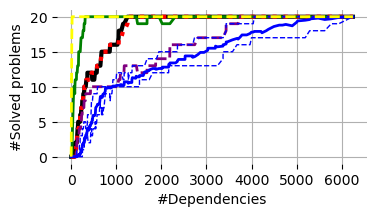
\includegraphics[width=1\linewidth]{Results_graphs/Joint_Projection/With_Random/coverage_Joint_Projection_Elevators}
  \caption{Elevators, max dep = 6245}
  \label{fig:Elevators}
\end{subfigure}\hspace{1em}
\begin{subfigure}[b]{0.3\textwidth}
\centering
  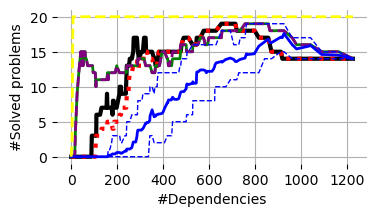
\includegraphics[width=1\linewidth]{Results_graphs/Joint_Projection/With_Random/coverage_Joint_Projection_BlocksWorld}
  \caption{Blocksworld, max dep = 1225}
  \label{fig:Blocksworld}
\end{subfigure}\hspace{1em}
\begin{subfigure}[b]{0.3\textwidth}
\centering
  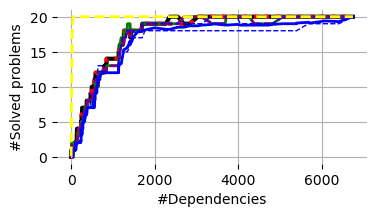
\includegraphics[width=1\linewidth]{Results_graphs/Joint_Projection/With_Random/coverage_Joint_Projection_Depot_not_trun}
  \caption{Depot, max dep = 6753}
  \label{fig:Depot}
\end{subfigure}\hspace{1em}
\begin{subfigure}[b]{0.3\textwidth}
\centering
  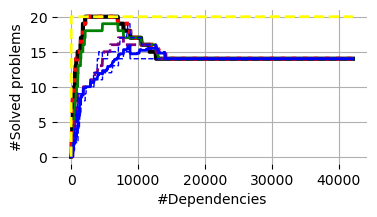
\includegraphics[width=1\linewidth]{Results_graphs/Joint_Projection/With_Random/coverage_Joint_Projection_Rovers}
  \caption{Rovers, max dep = 42155}
  \label{fig:Rovers}
\end{subfigure}\hspace{1em}
\begin{subfigure}[b]{0.3\textwidth}
\centering
  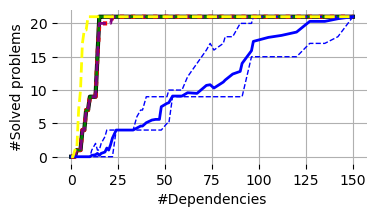
\includegraphics[width=1\linewidth]{Results_graphs/Joint_Projection/With_Random/coverage_Joint_Projection_Logistics}
  \caption{Logistics, max dep = 150}
  \label{fig:Logistics}
\end{subfigure}\hspace{1em}
\begin{subfigure}[b]{0.3\textwidth}
\centering
  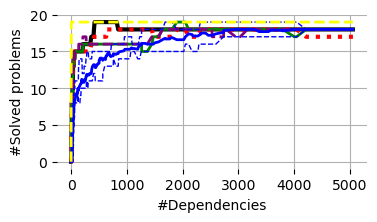
\includegraphics[width=1\linewidth]{Results_graphs/Joint_Projection/With_Random/coverage_Joint_Projection_Driverlog}
  \caption{Driverlog, max dep = 5060}
  \label{fig:Driverlog}
\end{subfigure}\hspace{1em}
\begin{subfigure}[b]{0.3\textwidth}
\centering
  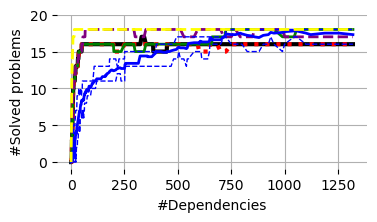
\includegraphics[width=1\linewidth]{Results_graphs/Joint_Projection/With_Random/coverage_Joint_Projection_ZenoTravel}
  \caption{ZenoTravel, max dep = 1320}
  \label{fig:ZenoTravel}
\end{subfigure}\hspace{1em}
\begin{subfigure}[b]{0.5\textwidth}
\centering
  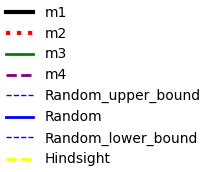
\includegraphics[scale=1]{Results_graphs/coverage_legend_with_random}
  \caption{Legend.}
  \label{fig:Legend}
\end{subfigure}\hspace{1em}
\caption{\# of solved problems for each amount of published dependencies in the Joint projection method.
\commentout{Graphs truncated after all methods solve all problems.}}
\label{fig:Coverage}
\end{figure*}

%Solved figure:
%Only MAFS graphs:
\begin{figure*}[t!]
\centering
\begin{subfigure}[b]{0.3\textwidth}
\centering
  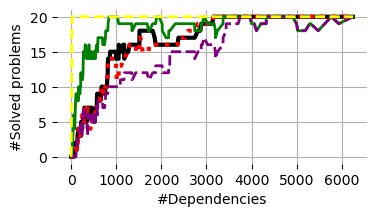
\includegraphics[width=1\linewidth]{Results_graphs/MAFS/coverage_MAFS_Elevators}
  \caption{Elevators, max dep = 6245}
  \label{fig:ElevatorsMAFS}
\end{subfigure}\hspace{1em}
\begin{subfigure}[b]{0.3\textwidth}
\centering
  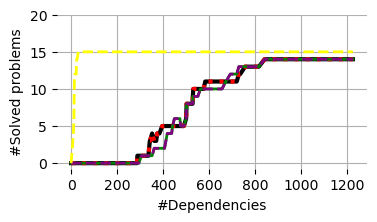
\includegraphics[width=1\linewidth]{Results_graphs/MAFS/coverage_MAFS_BlocksWorld}
  \caption{Blocksworld, max dep = 1225}
  \label{fig:BlocksworldMAFS}
\end{subfigure}\hspace{1em}
\begin{subfigure}[b]{0.3\textwidth}
\centering
  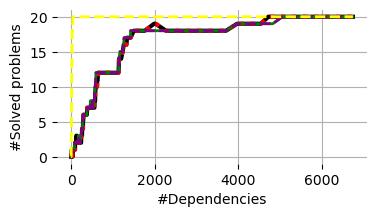
\includegraphics[width=1\linewidth]{Results_graphs/MAFS/coverage_MAFS_Depot}
  \caption{Depot, max dep = 6753}
  \label{fig:DepotMAFS}
\end{subfigure}\hspace{1em}
\begin{subfigure}[b]{0.3\textwidth}
\centering
  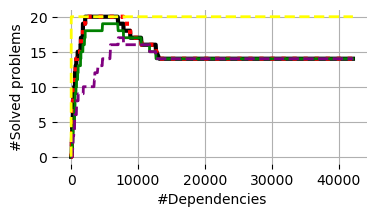
\includegraphics[width=1\linewidth]{Results_graphs/MAFS/coverage_MAFS_Rovers}
  \caption{Rovers, max dep = 42155}
  \label{fig:RoversMAFS}
\end{subfigure}\hspace{1em}
\begin{subfigure}[b]{0.3\textwidth}
\centering
  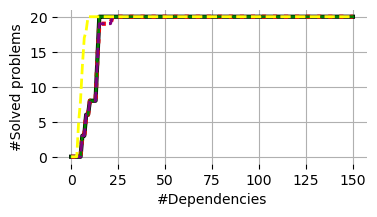
\includegraphics[width=1\linewidth]{Results_graphs/MAFS/coverage_MAFS_Logistics}
  \caption{Logistics, max dep = 150}
  \label{fig:LogisticsMAFS}
\end{subfigure}\hspace{1em}
\begin{subfigure}[b]{0.3\textwidth}
\centering
  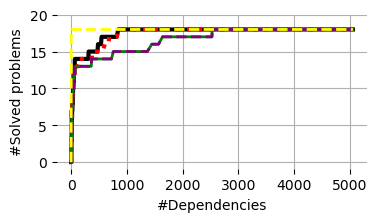
\includegraphics[width=1\linewidth]{Results_graphs/MAFS/coverage_MAFS_Driverlog}
  \caption{Driverlog, max dep = 5060}
  \label{fig:DriverlogMAFS}
\end{subfigure}\hspace{1em}
\begin{subfigure}[b]{0.3\textwidth}
\centering
  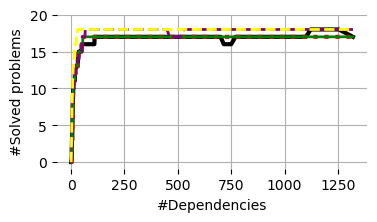
\includegraphics[width=1\linewidth]{Results_graphs/MAFS/coverage_MAFS_ZenoTravel}
  \caption{ZenoTravel, max dep = 1320}
  \label{fig:ZenoTravelMAFS}
\end{subfigure}\hspace{1em}
\begin{subfigure}[b]{0.5\textwidth}
\centering
  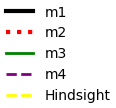
\includegraphics[scale=1]{Results_graphs/coverage_legend_without_random}
  \caption{Legend.}
  \label{fig:LegendMAFS}
\end{subfigure}\hspace{1em}
\caption{\# of solved problems for each amount of published dependencies in the \mafs method.
\commentout{Graphs truncated after all methods solve all problems.}}
\label{fig:CoverageMAFS}
\end{figure*}


%Dependencies graphs:
\begin{figure*}[t!]
\centering
\begin{subfigure}[b]{0.3\textwidth}
\centering
  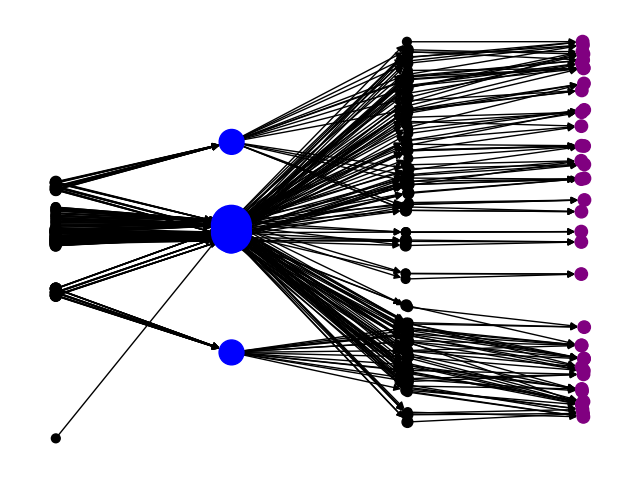
\includegraphics[width=1\linewidth]{Dependencies_graphs/DepGraphElevators}
  \caption{Elevators}
  \label{fig:DepGraphElevators}
\end{subfigure}\hspace{1em}
\begin{subfigure}[b]{0.3\textwidth}
\centering
  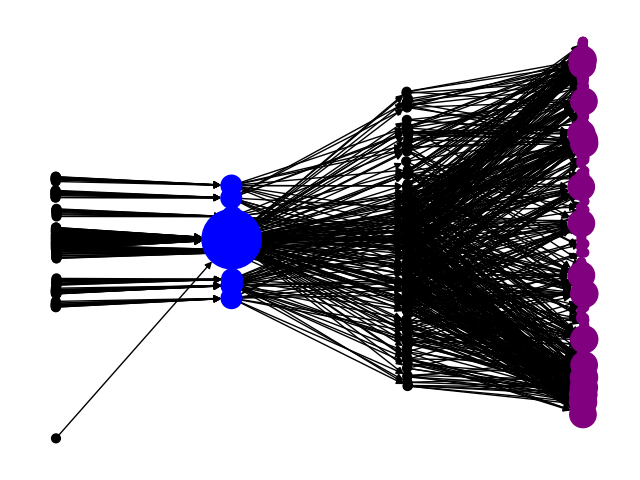
\includegraphics[width=1\linewidth]{Dependencies_graphs/DepGraphBlocksWorld}
  \caption{BlocksWorld}
  \label{fig:DepGraphBlocksWorld}
\end{subfigure}\hspace{1em}
\begin{subfigure}[b]{0.3\textwidth}
\centering
  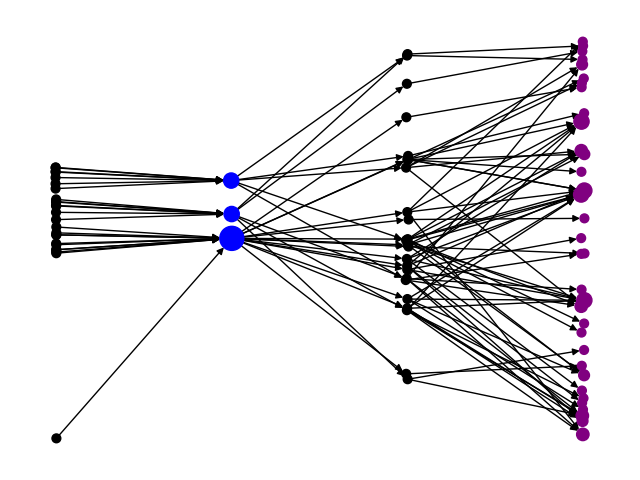
\includegraphics[width=1\linewidth]{Dependencies_graphs/DepGraphDepot}
  \caption{Depot}
  \label{fig:DepGraphDepot}
\end{subfigure}\hspace{1em}
\begin{subfigure}[b]{0.3\textwidth}
\centering
  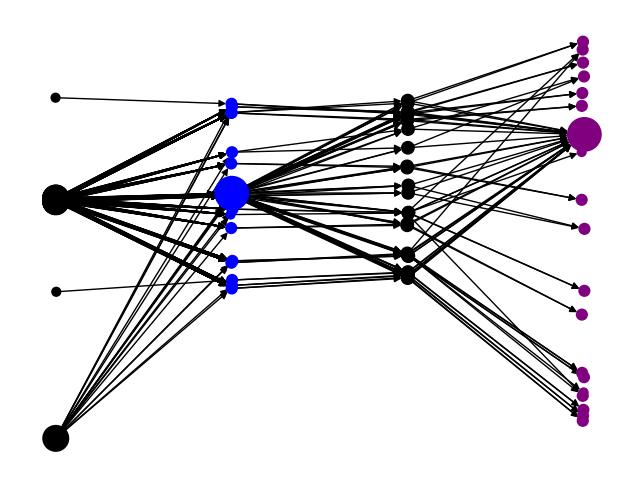
\includegraphics[width=1\linewidth]{Dependencies_graphs/DepGraphRovers}
  \caption{Rovers}
  \label{fig:DepGraphRovers}
\end{subfigure}\hspace{1em}
\begin{subfigure}[b]{0.3\textwidth}
\centering
  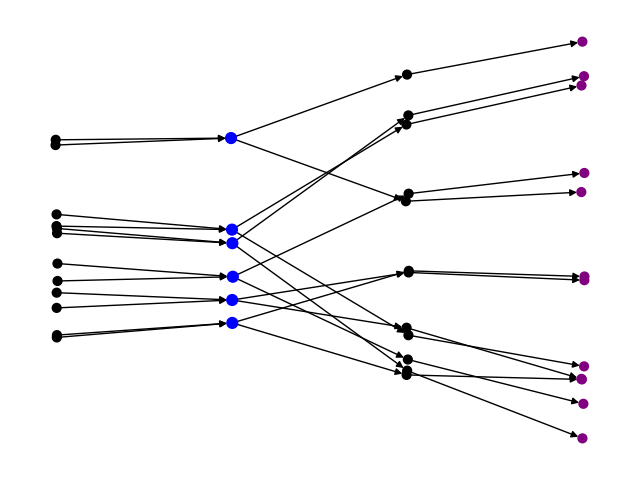
\includegraphics[width=1\linewidth]{Dependencies_graphs/DepGraphLogistics}
  \caption{Logistics}
  \label{fig:DepGraphLogistics}
\end{subfigure}\hspace{1em}
\begin{subfigure}[b]{0.3\textwidth}
\centering
  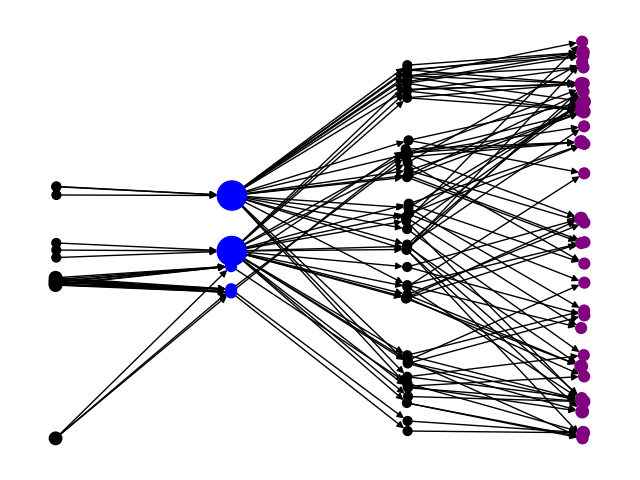
\includegraphics[width=1\linewidth]{Dependencies_graphs/DepGraphDriverlog}
  \caption{Driverlog}
  \label{fig:DepGraphDriverlog}
\end{subfigure}\hspace{1em}
\begin{subfigure}[b]{0.3\textwidth}
\centering
  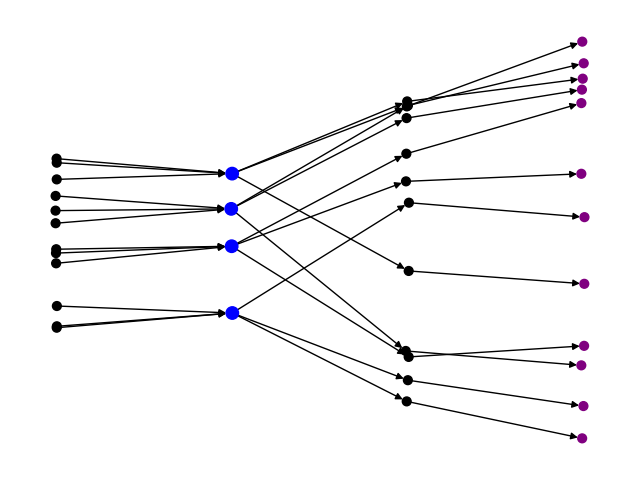
\includegraphics[width=1\linewidth]{Dependencies_graphs/DepGraphZenoTravel}
  \caption{ZenoTravel}
  \label{fig:DepGraphZenoTravel}
\end{subfigure}\hspace{1em}
\caption{Single agent dependency graphs for all domains. All of the dependencies graphs are drawn for the easiest problem of the domain. Each dependencies graph has the same layers as described previously. The size of the nodes in the first and second layers, is their \emph{out-degree}, and the size of the nodes in the third and fourth layers is their \emph{in-degree}. There is also a special action that is a dummy-init-action in each domain, that action is at the bottom of the first actions layer. The dummy-init-action does not appear in Logistics and ZenoTravel, because it does not have any dependency with another public action in these domains.}
\label{fig:DependenciesGraphs}
\end{figure*}






%New cost table:
% Please add the following required packages to your document preamble:
% \usepackage{multirow}
\begin{table*}[ht]
\begin{tabular}{|c|c|c|c|c|c|c||c|c|c|c|c|}
\hline
\multirow{2}{*}{\textbf{Domain}} & \multirow{2}{*}{\textbf{M}} & \multicolumn{5}{c||}{\textbf{Joint projection}}                                       & \multicolumn{5}{c|}{\textbf{MAFS}}                                                    \\ \cline{3-12} 
                                 &                             & \textbf{Min} & \textbf{Max} & \textbf{Min. dep} & \textbf{Max. dep} & \textbf{Imp.}    & \textbf{Min} & \textbf{Max} & \textbf{Min. dep} & \textbf{Max. dep} & \textbf{Imp.}   \\ \hline
\multirow{4}{*}{BlocksWorld}     & m1                          & 48.95        & 111.75       & 92.10             & 55.15             & 45.39\%          & 29.33        & 30.93        & 30.07             & 30.20             & \textbf{1.93\%} \\ \cline{2-12} 
                                 & m2                          & 51.15        & 95.65        & 79.50             & 55.15             & \textbf{36.25\%} & 29.33        & 30.93        & 30.07             & 30.20             & \textbf{1.93\%} \\ \cline{2-12} 
                                 & m3                          & 47.35        & 99.65        & 83.20             & 50.10             & 43.05\%          & 28.57        & 31.64        & 29.57             & 30.64             & 2.98\%          \\ \cline{2-12} 
                                 & m4                          & 47.65        & 97.95        & 81.60             & 50.10             & 42.61\%          & 28.57        & 31.64        & 29.57             & 30.64             & 2.98\%          \\ \hline
\multirow{4}{*}{Depot}           & m1                          & 21.35        & 29.50        & 28.75             & 21.55             & 21.61\%          & 21.15        & 21.70        & 21.25             & 21.55             & 1.13\%          \\ \cline{2-12} 
                                 & m2                          & 21.35        & 29.45        & 28.40             & 21.55             & 19.73\%          & 21.15        & 21.65        & 21.20             & 21.55             & \textbf{0.71\%} \\ \cline{2-12} 
                                 & m3                          & 21.45        & 28.90        & 28.45             & 21.55             & \textbf{19.18\%} & 21.25        & 21.65        & 21.30             & 21.55             & \textbf{0.71\%} \\ \cline{2-12} 
                                 & m4                          & 21.45        & 29.05        & 28.60             & 21.55             & 20.26\%          & 21.25        & 21.65        & 21.30             & 21.55             & \textbf{0.71\%} \\ \hline
\multirow{4}{*}{Driverlog}       & m1                          & 28.89        & 63.63        & 61.42             & 29.32             & 32.82\%          & 21.11        & 23.56        & 22.39             & 22.67             & 6.48\%          \\ \cline{2-12} 
                                 & m2                          & 22.22        & 43.61        & 41.28             & 22.67             & 30.10\%          & 21.61        & 23.50        & 22.61             & 22.67             & 5.91\%          \\ \cline{2-12} 
                                 & m3                          & 39.21        & 58.63        & 57.00             & 39.47             & \textbf{23.98\%} & 21.17        & 23.39        & 22.17             & 22.67             & 5.91\%          \\ \cline{2-12} 
                                 & m4                          & 22.44        & 46.33        & 44.61             & 22.67             & 28.31\%          & 21.17        & 23.39        & 22.06             & 22.67             & \textbf{5.55\%} \\ \hline
\multirow{4}{*}{Elevators}       & m1                          & 33.50        & 53.10        & 37.45             & 46.90             & \textbf{10.67\%} & 37.25        & 61.75        & 39.90             & 55.70             & 6.88\%          \\ \cline{2-12} 
                                 & m2                          & 33.55        & 54.45        & 39.15             & 46.90             & 16.08\%          & 39.35        & 61.40        & 42.65             & 55.70             & 9.67\%          \\ \cline{2-12} 
                                 & m3                          & 33.00        & 51.25        & 38.35             & 46.90             & 13.38\%          & 33.60        & 58.90        & 36.10             & 55.70             & \textbf{6.36\%} \\ \cline{2-12} 
                                 & m4                          & 34.75        & 51.75        & 38.35             & 46.90             & 10.20\%          & 37.55        & 60.50        & 40.90             & 55.70             & 9.19\%          \\ \hline
\multirow{4}{*}{Logistics}       & m1                          & 25.05        & 31.29        & 27.24             & 29.24             & 6.40\%           & 25.15        & 31.95        & 27.85             & 29.35             & 8.04\%          \\ \cline{2-12} 
                                 & m2                          & 25.05        & 31.29        & 26.81             & 29.24             & \textbf{5.33\%}  & 25.15        & 31.95        & 27.35             & 29.35             & \textbf{6.75\%} \\ \cline{2-12} 
                                 & m3                          & 25.00        & 31.24        & 27.24             & 29.24             & 6.62\%           & 25.15        & 31.95        & 27.85             & 29.35             & 8.07\%          \\ \cline{2-12} 
                                 & m4                          & 25.00        & 31.24        & 26.81             & 29.24             & 5.55\%           & 25.15        & 31.95        & 27.35             & 29.35             & 6.79\%          \\ \hline
\multirow{4}{*}{Rovers}          & m1                          & 49.50        & 53.00        & 52.40             & 50.25             & 6.07\%           & 57.50        & 62.30        & 61.45             & 58.35             & 8.12\%          \\ \cline{2-12} 
                                 & m2                          & 50.25        & 51.50        & 51.50             & 50.25             & \textbf{3.28\%}  & 58.25        & 60.40        & 60.40             & 58.35             & \textbf{4.99\%} \\ \cline{2-12} 
                                 & m3                          & 51.74        & 68.42        & 67.58             & 52.84             & 22.68\%          & 60.26        & 83.05        & 82.00             & 62.37             & 26.83\%         \\ \cline{2-12} 
                                 & m4                          & 51.53        & 64.35        & 63.35             & 52.53             & 18.26\%          & 58.00        & 77.41        & 77.41             & 58.41             & 24.41\%         \\ \hline
\multirow{4}{*}{ZenoTravel}      & m1                          & 45.12        & 56.12        & 47.59             & 54.41             & 9.32\%           & 52.44        & 63.11        & 55.00             & 61.28             & 8.96\%          \\ \cline{2-12} 
                                 & m2                          & 37.31        & 50.63        & 39.81             & 48.81             & 9.81\%           & 44.06        & 56.53        & 46.65             & 54.59             & 9.39\%          \\ \cline{2-12} 
                                 & m3                          & 51.83        & 62.83        & 54.61             & 60.72             & \textbf{8.69\%}  & 45.24        & 56.71        & 47.94             & 54.59             & 9.06\%          \\ \cline{2-12} 
                                 & m4                          & 51.83        & 62.83        & 54.61             & 60.72             & \textbf{8.69\%}  & 52.33        & 63.39        & 55.11             & 61.28             & \textbf{8.69\%} \\ \hline \hline
\multirow{4}{*}{Average}         & m1                          & 36.05        & 56.91        & 49.56             & 40.97             & 18.90\%          & 34.85        & 42.19        & 36.84             & 39.87             & 5.93\%          \\ \cline{2-12} 
                                 & m2                          & 34.41        & 50.94        & 43.78             & 39.22             & \textbf{17.23\%} & 34.13        & 40.91        & 35.85             & 38.91             & \textbf{5.62\%} \\ \cline{2-12} 
                                 & m3                          & 38.51        & 57.27        & 50.92             & 42.98             & 19.66\%          & 33.61        & 43.90        & 38.13             & 39.55             & 8.56\%          \\ \cline{2-12} 
                                 & m4                          & 36.38        & 54.79        & 48.28             & 40.53             & 19.13\%          & 34.86        & 44.28        & 39.10             & 39.94             & 8.33\%          \\ \hline
\end{tabular}
\caption{Averaged plan makespan cost over all of solved problems for each domain. Min denotes the average minimal cost over all solved problems.
Max denotes the average maximal cost.
Min. dep denotes the cost when solved with the minimal amount of disclosed dependencies.
Max. dep denotes the cost when solved with the maximal amount of disclosed dependencies.
Imp. denotes improvement between the first time that the problem was solved to the best achieved solution.
The lowest improvement, and hence best initial plan, is in bold.}
%(calculated by the following formula: $\frac{First \, solved \, cost - Minimal \, cost}{First \, solved \, cost}*100\%$)}
\label{table:costTable}
\end{table*}


Here, we provide an extended and more detailed version of our experimental results. 
Details regarding the experimental setup are given in the main article. 

Namely, Figure~\ref{fig:Coverage} shows the number of problems that were solved on each domain given the number of revealed dependencies by each agent in the projection-based solver.
Figure~\ref{fig:CoverageMAFS} shows the number of problems that were solved on each domain given the number of revealed dependencies by each agent using \mafs.
Figure~\ref{fig:DependenciesGraphs} shows agent's dependency graphs, as described in the main article.
Table~\ref{table:costTable} shows the results of the following averaged factors: (1) Min. cost, (2) Max. cost, (3) Min. dep. cost --- the solution cost for a plan found with the least amount of revealed dependencies, 
and (4) Max. dep. cost -- the solution cost for a plan that was found with the maximal amount of dependencies revealed.
The ``Improvement'' column  shows  the percentage of the minimal cost out of the Min. dep. cost $(\frac{Min. \, dep. \, cost - Min. \, cost}{Min. \, dep. \, cost}*100\%)$. That is, how much cost can be reduced by revealing more dependencies. 
The trends observed in all these results are discussed in the main article.

\newpage
%\bibliographystyle{ACM-Reference-Format} 
\bibliographystyle{named}
\bibliography{biblio}

\end{document}
